\documentclass[tikz,border=4pt]{standalone}
\usepackage{amsmath}
\begin{document}
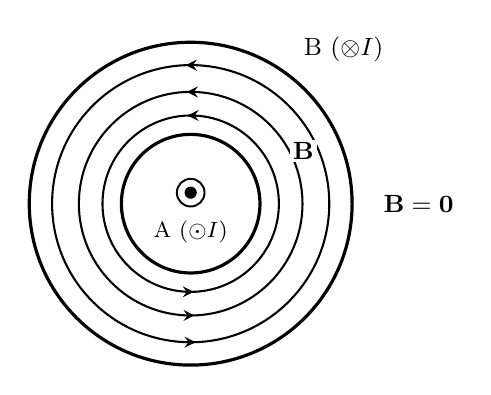
\begin{tikzpicture}[>=stealth, thick, scale=1.0]
  % Inner cylinder A (radius a = 0.88) and outer cylinder B (radius b = 2.05)
  \draw[line width=1.15pt] (0, 0) circle (0.88);
  \draw[line width=1.15pt] (0, 0) circle (2.05);

  % Concentric CCW magnetic field circles in a < r < b
  \foreach \rad in {1.12, 1.42, 1.76} {
    \draw[line width=0.75pt] (0, 0) circle (\rad);
    \draw[->, line width=0.75pt] (88:\rad) -- (92:\rad);
    \draw[->, line width=0.75pt] (268:\rad) -- (272:\rad);
  }

  % Current direction symbol inside A
  \fill (0, 0.14) circle (2.2pt);
  \draw[line width=0.7pt] (0, 0.14) circle (5pt);
  \node[font=\footnotesize] at (0, -0.36) {$\mathrm{A}\ (\odot I)$};

  \node[above right, font=\small] at (52:2.12) {$\mathrm{B}\ (\otimes I)$};
  \node[font=\small, fill=white, inner sep=1pt] at (25:1.58) {$\mathbf{B}$};
  \node[right, font=\small] at (2.32, 0) {$\mathbf{B} = \mathbf{0}$};
\end{tikzpicture}
\end{document}
